\documentclass[12pt]{article}

\usepackage[utf8]{inputenc}
\usepackage[T1]{fontenc}
\usepackage{amsmath,amssymb}
\usepackage{graphicx}
\usepackage{booktabs}
\usepackage{hyperref}
\usepackage[round]{natbib}
\usepackage{xcolor}
\usepackage[margin=1in]{geometry}
\usepackage{tikz}
\usetikzlibrary{arrows.meta, positioning, decorations.markings}

\title{Narcissus: How AI Mirrors Amplify Researcher Confirmation Bias}
% AUTHOR-ANONYMIZED for double-blind submission.
% Camera-ready identity: Heznpc (Independent Researcher, contact: heznpc@gmail.com).
\author{Anonymous Author(s)\\
Affiliation withheld for blind review}
\date{}

\begin{document}
\maketitle

\begin{abstract}
When researchers use AI assistants for real-time literature search and writing simultaneously, a positive feedback loop emerges that we term \textbf{collaborative entrenchment}. The researcher's thesis biases the AI's search and interpretation; the AI's outputs reinforce the researcher's framing; and accumulated context ensures that each subsequent interaction deepens the alignment. This phenomenon is distinct from either human confirmation bias or AI sycophancy alone---it is an emergent property of the interaction loop that neither agent would produce in isolation. We present empirical evidence from a natural experiment in which five academic papers were reviewed under three conditions: a Deep session carrying full conversation history, Fresh Agent sessions with zero prior context assigned as adversarial reviewers, and a Separate Session operating independently. The Deep session systematically missed six critical problems that context-free sessions detected. A citation audit flagged four AI-suggested citations with suspect attribution; on external two-directional verification, two are confirmed directional author-misattributions (correct papers paired with the names of real, domain-adjacent scholars who did not write them), one is an institutional/format discrepancy, and the fourth has an attribution we could not verify in either direction; separately, five AI-suggested citations uniformly strengthened the thesis with zero counter-arguments surfaced. A reference audit of one paper found author-attribution errors in 9 of 11 flagged references. We formalize this feedback cycle as the \textbf{Narcissus Loop}, distinguish it from known cognitive and machine biases, explain why context-free review sessions break the loop, and propose both an observational case study using git history and a controlled $2 \times 2$ experiment for systematic validation. Our findings suggest that AI-assisted research requires architectural safeguards---not merely researcher awareness---to prevent collaborative entrenchment from compromising scholarly rigor.
\end{abstract}

%----------------------------------------------------------------------
\section{Introduction}
\label{sec:introduction}

The integration of large language models (LLMs) into academic research workflows has accelerated rapidly. Researchers now routinely use AI assistants for literature discovery, conceptual exploration, draft composition, and iterative refinement---often within a single, continuous session \citep{lee2022, gero2023}. This integration offers genuine advantages: broader literature coverage, faster iteration cycles, and the capacity to maintain coherent arguments across complex multi-source analyses. Yet these advantages share a mechanism with a subtle and compounding failure mode.

The core claim of this paper is as follows. When a researcher uses an AI assistant for real-time literature search and writing simultaneously, a specific feedback loop emerges: the researcher's existing framing biases the AI's search and interpretation, and the AI's contextually coherent outputs reinforce the researcher's framing. Over the course of a working session, the AI's context window accumulates material aligned with the researcher's thesis, which progressively biases subsequent outputs toward further confirmation. We call this phenomenon \textbf{collaborative entrenchment}.

Collaborative entrenchment is not simply confirmation bias assisted by a compliant tool. Confirmation bias \citep{nickerson1998} is a well-documented property of individual human cognition---the tendency to seek, interpret, and recall information that confirms pre-existing beliefs. AI sycophancy \citep{perez2022, sharma2023} is a separately documented property of language models---the tendency to agree with the user's stated position. Collaborative entrenchment is distinct from both because it is an emergent property of the \emph{interaction loop} between two agents. The human biases the query; the model biases the response; the biased response enters the context window; the enriched context biases the next response further. Neither the human's confirmation bias nor the model's sycophantic tendency alone would produce the compounding trajectory that their interaction generates.

This distinction matters practically. Interventions targeting confirmation bias (e.g., debiasing training, awareness campaigns) address the human agent. Interventions targeting sycophancy (e.g., RLHF penalties for agreement, constitutional AI constraints) address the model agent. Neither addresses the loop itself. As we show empirically, a researcher who had explicitly theorized this mechanism---who had named it, written about it, and designed countermeasures---still fell victim to it. Knowing about collaborative entrenchment did not prevent collaborative entrenchment. This suggests that effective mitigation must be \emph{architectural}, not merely epistemic.

The paper is organized as follows. Section~\ref{sec:evidence} presents empirical evidence from a natural experiment involving three independent review sessions of the same papers under different context conditions, supplemented by citation and reference audits. Section~\ref{sec:mechanism} formalizes the Narcissus Loop as a feedback cycle, distinguishes it from known biases, and explains why context-free sessions break the loop. Section~\ref{sec:study-design} proposes two study designs for systematic validation. Section~\ref{sec:implications} discusses implications for research practice, AI system design, and the broader Ploidy research program on context-asymmetric debate. Sections~\ref{sec:related} and~\ref{sec:limitations} address related work and limitations, respectively.

A note on scope: a companion paper provides a first-person reflexive account of using LLM infrastructure across a multi-project research program, documenting the experiential arc of amplification, degradation, and correction. The present paper is deliberately different in register. Where the reflexive account asks \emph{what it felt like}, this paper asks \emph{what the data show}. The evidence base, analytical framework, and proposed study designs are intended to make collaborative entrenchment an empirically testable claim rather than a phenomenological observation.

%----------------------------------------------------------------------
\section{Evidence}
\label{sec:evidence}

The evidence presented in this section derives from a natural experiment that arose during the development of a multi-project research portfolio. Five academic papers spanning HCI, NLP, philosophy, media studies, and cultural anthropology were developed using a single AI assistant (Claude Opus 4.6, frontier model at the time of the audit in 2026-Q1) as the primary research infrastructure---handling literature search, framework development, draft composition, and iterative revision within continuous sessions. The same model was subsequently used under three distinct context conditions to review the resulting papers. The conditions were not designed as an experiment \textit{a priori}; they emerged from the practical workflow of seeking different forms of feedback. Their systematic comparison, however, reveals patterns consistent with collaborative entrenchment.

A successor model (Claude Opus 4.7) was released in 2026-Q2, after the audit was complete. We preserve the 4.6-frozen audit as the natural-experiment record and add a model-version replication arm to Study~1 (Section~\ref{sec:study1}) and a model-version covariate to Study~2 (Section~\ref{sec:study2}) to test whether the observed effects are specific to a single model version or persist across the version boundary.

\subsection{Three-Session Natural Experiment}
\label{sec:three-session}

Each of the five papers was reviewed under three conditions that differed in context depth and assigned role (Table~\ref{tab:sessions}).

\begin{table}[htbp]
\centering
\caption{Three-session comparison: context depth and role assignment.}
\label{tab:sessions}
\begin{tabular}{lll}
\toprule
Session & Context Depth & Role \\
\midrule
Deep & Full conversation history (hours) & Primary collaborator \\
Fresh Agents & Zero context, raw paper files only & Adversarial reviewers \\
Separate Session & Zero context, independent instance & Independent reviewer \\
\bottomrule
\end{tabular}
\end{table}

The \textbf{Deep session} was the primary working environment: a long-running conversation in which the AI had participated in literature search, framework development, and draft composition for each paper. By the time review occurred, the context window contained hours of thesis-aligned material. The \textbf{Fresh Agent} sessions were spawned with zero prior context, given only the raw paper files, and explicitly instructed to act as adversarial reviewers tasked with identifying weaknesses. The \textbf{Separate Session} was an independent instance with no prior context and no adversarial instruction---simply asked to review the papers on their merits.

\textbf{Caveat: Confounds in the natural experiment.} The three conditions differ on at least four dimensions simultaneously: context depth (hours of accumulated history vs.\ none), assigned role (collaborator vs.\ adversarial reviewer vs.\ independent reviewer), prompt wording, and review timing. The Fresh Agents' adversarial instruction in particular is a confound that cannot be attributed to context depth alone. We therefore treat the data below as a \emph{single-program existence proof} that motivates the controlled design in Section~\ref{sec:study2}, not as a clean isolation of context depth. The factorial design of Study~2 separates context depth from assigned role.

\textbf{Partial isolation of the adversarial-framing confound (2026-05-21 stance comparison).} A direct adversarial-vs-neutral comparison was conducted on the same five papers (5 runs per stance, claude-opus-4-6, 50 cells total). Total per-cell issue count was essentially unchanged ($-5\%$ on average across the five papers; range $-15\%$ to $+18\%$, with ploidy as the lone positive outlier). What changed substantially was the severity distribution: across the cohort, critical-tier issues dropped from 62 to 38 ($-39\%$) and minor-tier issues rose from 94 to 129 ($+37\%$) under neutral framing. Stable-core sections (those flagged by all five runs at a given stance) overlapped substantially between stances (14 of 19 unioned stable sections appeared in both stance cores), and the neutral cores were predominantly subsets of the adversarial cores. The interpretation: adversarial framing inflates the \emph{severity weight} of detected concerns but does not cause detection of structural concerns the neutral reviewer misses. The \emph{what is flagged} signal in Table~\ref{tab:findings} is therefore robust to stance; the absolute severity-tier labels are stance-dependent and should be read accordingly.

\textbf{Inclusion criteria for the findings reported below.} Table~\ref{tab:findings} reports every issue raised by \emph{at least one} of the three sessions during review, classified by which session(s) detected it. Issues raised by the Deep session alone (i.e., problems the Fresh and Separate sessions missed) would also appear in this table; \textbf{no such issues were identified} during the review process. We acknowledge that this absence is itself evidence consistent with the Deep session's confirmation-aligned stance and cannot independently rule out a selection effect; the controlled design of Study~2 (Section~\ref{sec:study2}) addresses this through blinded reviewer ratings of cells, where Deep-only detections, if they exist, would surface as Deep-condition advantages on independent rubric items.

Table~\ref{tab:findings} summarizes the key divergences across sessions.

\begin{table}[htbp]
\centering
\caption{Key findings across sessions. Deep session systematically aligned with author framing; fresh sessions were independently critical but caught different subsets of problems.}
\label{tab:findings}
\begin{tabular}{p{5cm}lll}
\toprule
Finding & Deep & Fresh Agent & Separate \\
\midrule
Z-Gap P3/P2 English-pivot double standard & Missed & Caught & Caught \\
Z-Gap $R_{\text{code}}=1.04$ too weak for claims & Accepted & ``Noise-level'' & Partially \\
Analogic: Era 2 isn't appropriation (de Certeau) & Missed & Caught & Missed \\
Analogic: D\&D/TTRPG diffusion path & Missed & Caught & Missed \\
Eddy: novelty decay vs.\ compound advantage & Missed & Not reviewed & Caught \\
Ploidy: Husserl epoch\'e $\neq$ passive memory absence & Missed & Not reviewed & Caught \\
\bottomrule
\end{tabular}
\end{table}

Three patterns in Table~\ref{tab:findings} merit attention.

First, \textbf{the Deep session missed every problem that the context-free sessions caught}. Across six identified issues spanning five papers, the Deep session detected none. This is not a sampling artifact---the Deep session reviewed the same material and had strictly more information available than either context-free session. The information asymmetry ran in the Deep session's favor; the critical detection ran against it.

Second, \textbf{the two context-free sessions caught different subsets of problems}. The Fresh Agent sessions, instructed as adversarial reviewers, identified the Z-Gap double standard and the Analogic misapplication of de Certeau's framework. The Separate Session, operating without adversarial instruction, caught the Eddy novelty-decay tension and the Ploidy Husserl mischaracterization. This complementarity suggests that context freedom is necessary but not sufficient---the assigned role and the reviewer's own interpretive orientation determine which problems surface. No single session caught all six issues.

Third, \textbf{the Deep session's failures were systematic, not random}. The missed problems share a structural feature: each would have required the reviewer to challenge a framing assumption that had been collaboratively established during the writing process. The Z-Gap double standard required questioning whether the paper applied its own analytical framework consistently. The Analogic de Certeau issue required questioning whether the theoretical lens fit the evidence. The Deep session, having participated in constructing these framings, evaluated the papers from within the frame rather than examining the frame itself. This is the behavioral signature of collaborative entrenchment: the accumulated context becomes the lens through which the paper is evaluated, rendering the lens itself invisible.

\subsection{AI-Hallucinated Citation Attribution}
\label{sec:hallucinated-citations}

During the collaborative writing process, the AI assistant suggested citations to support specific claims. A post-hoc verification audit flagged four cases in which the cited author attribution appeared to diverge from the real paper's authorship (Table~\ref{tab:hallucinated}). On external two-directional verification (confirming the real author \emph{and} searching for a competing paper under the cited name), two are confirmed author-misattributions (citations 1--2), one is an institutional/format discrepancy rather than an author hallucination (citation 3), and the fourth (the ``memetic performance'' citation) could not be verified in either direction and is retained as \emph{unverified} rather than asserted as fabricated---``could not find it'' is not ``confirmed fabricated,'' which would be the inverse of the very error this paper studies.

\begin{table}[htbp]
\centering
\caption{AI-suggested citation metadata under audit. Papers exist; the cited author differs from the verified author in three cases (citations 1--3) and is unverifiable in one (citation 4, marked unverified).}
\label{tab:hallucinated}
\begin{tabular}{p{3cm}p{3cm}p{3cm}l}
\toprule
Citation & AI-Suggested Author & Actual Author & Paper Exists? \\
\midrule
12-LMIC play study & Atabey, D. & Iannelli, O. et al. & Yes \\
Folk in Age of Algorithms & Blank, T.J. \& Kitta, A. & Flinterud, G. & Yes \\
Roblox Indonesia & (correct institution) & (blog post, not report) & Yes \\
Memetic performance & Melo, G.S. & (unverified) & Yes \\
\bottomrule
\end{tabular}
\end{table}

The hallucination pattern is notable for what it is \emph{not}. These are not wholesale fabrications---fictitious papers conjured to fill a citation need. In every case, the AI located a real paper that genuinely supported the claim being made. The hallucination occurred at the metadata level: the AI generated plausible-sounding author names drawn from the same research domain rather than retrieving the actual attribution. Atabey is a real researcher in childhood studies; Blank and Kitta are real folklorists. The fabricated names were not random---they were \emph{domain-coherent}, suggesting that the model's generation process prioritized contextual plausibility over factual accuracy.

This directional hallucination pattern carries a specific implication for collaborative entrenchment. When an AI fabricates metadata for a real paper that supports the researcher's thesis, the resulting citation \emph{looks correct on every dimension that the researcher is likely to check}. The paper exists. The claim it supports is accurate. The author name sounds right for the field. Only a systematic metadata verification---checking the actual author list against the cited name---reveals the error. In a workflow where the researcher trusts the AI's citation suggestions because prior suggestions have been substantively accurate, these metadata errors pass through undetected. The trust is locally rational (the paper and the claim are real) but globally corrosive (the citation record is corrupted).

\subsection{Directional Citation Bias}
\label{sec:directional-bias}

A git diff analysis of citation additions across the collaborative writing process revealed a pronounced directional asymmetry. In the Analogic paper on play appropriation, five citations were added during AI-assisted local refinement sessions. All five strengthened the paper's central thesis. Zero counter-arguments or qualifying citations were introduced during the same period. Separately, three interpretive hypotheses were added to the Z-Gap paper's analysis of cross-linguistic code-mixing patterns, each functioning to rescue the main thesis from ambiguous data. Again, zero alternative interpretations were proposed by the AI during the collaborative writing process.

This asymmetry persisted until a context-free review was explicitly requested. When Fresh Agent sessions reviewed the same papers, the asymmetry reversed sharply. Within minutes, the Fresh Agent identified three counter-citations for the Analogic paper---works by Nielsen (2012) on participatory appropriation, Mustola (2018) on children's digital agency, and Lancy (2015) on cross-cultural play norms---that directly challenged or substantially qualified the paper's claims. For the Z-Gap paper, the Fresh Agent identified eight missing critical references, including foundational works by Joshi (1985) on code-switching constraints, Conneau et al.\ (2020) on cross-lingual transfer learning, and Fine (1983) on shared knowledge in interaction, among others.

The pattern is consistent with collaborative entrenchment operating at the citation level. During the collaborative writing process, the AI's literature search was conditioned on the accumulated thesis-aligned context. When asked to find supporting literature or strengthen an argument, the AI searched within the thesis's framing and returned confirming results. Counter-evidence was not suppressed---it was never searched for, because the search space was defined by the thesis. When a context-free session approached the same papers without accumulated framing, the search space expanded to include the broader literature, and counter-evidence appeared immediately.

The 5:0 ratio (thesis-supporting to counter-argument citations) in a single paper is a small sample, and directional citation bias could reflect researcher prompting behavior rather than AI-initiated bias. \textbf{All citation classifications reported in this section were performed by a single rater (the first author); inter-rater reliability was not measured. Study~1 (Section~\ref{sec:study1}) re-runs the classification with two blinded raters and reports Cohen's $\kappa$.} The figures below are therefore reported as exploratory effect-size estimates rather than as confirmatory measurements. However, the fact that the same AI model, given the same papers but without accumulated context, immediately produced counter-citations suggests that the Deep session's failure to surface counter-evidence was at least partially a function of context accumulation rather than model incapacity.

\subsection{Z-Gap Reference Audit: Systematic Placeholder Pattern}
\label{sec:reference-audit}

A systematic audit of the Z-Gap paper's reference list, conducted after the three-session comparison raised concerns about citation integrity, revealed a pervasive pattern of metadata degradation. Of 11 references flagged for verification, 9 contained author-attribution errors. The errors fell into three categories:

\begin{itemize}
    \item \textbf{Fabricated placeholder names} (4 cases): The paper title or a keyword from the abstract was used as the author name. For example, a paper on cross-linguistic transfer was attributed to an author whose ``name'' was derived from the paper's title rather than its actual author list.
    \item \textbf{Wrong author names} (3 cases): A real researcher's name was attached to a paper they did not write, mirroring the domain-coherent hallucination pattern observed in Table~\ref{tab:hallucinated}. The substituted names were plausible---researchers active in adjacent subfields---but incorrect.
    \item \textbf{Anonymous or missing attribution} (2 cases): The citation omitted author names entirely, listing only the institutional source or leaving the author field effectively blank.
\end{itemize}

In all 9 cases, the cited paper existed and the substantive claim it was cited to support was accurate. The degradation was confined to metadata: who wrote the paper, not what the paper said. This pattern reinforces the finding from Section~\ref{sec:hallucinated-citations}---the AI reliably identifies relevant literature but unreliably attributes it. From the standpoint of collaborative entrenchment, the pattern is significant because metadata errors are the errors least likely to be caught during normal research workflow. A researcher reviewing a draft checks whether the cited claim is supported by the cited source; checking whether the cited source is attributed to the correct author requires a separate verification step that is rarely performed during iterative writing.

The 9/11 error rate in a single paper's reference list is suggestive but cannot establish that the problem is systematic from a sample of one. We report it as motivating evidence for the systematic verification protocol in Study~1 (Section~\ref{sec:study1}), which extends metadata verification to every AI-suggested citation across all five papers and computes the rate against a published baseline for human-only citation practices. If a similar rate were to generalize across AI-assisted academic writing, it would imply that a non-trivial fraction of AI-suggested citations in the broader literature may carry corrupted metadata---a form of silent scholarly pollution that is invisible to readers who do not independently verify every reference---but establishing such generalization is left for prospective replication.

%----------------------------------------------------------------------
\section{Mechanism: The Narcissus Loop}
\label{sec:mechanism}

The evidence presented in Section~\ref{sec:evidence} is consistent with a feedback cycle that we term the \textbf{Narcissus Loop}, after the mythological figure who mistook his own reflection for another. In the Narcissus Loop, the researcher encounters the AI's outputs as external validation when they are, in significant part, reflections of the researcher's own framing filtered through the model's coherence optimization.

The loop operates through the following stages:

\begin{enumerate}
    \item \textbf{Thesis formation.} The researcher begins with a thesis $T$---an explanatory framework, a hypothesis, or a directional claim.
    \item \textbf{Framed search.} The researcher queries the AI for supporting literature, evidence, or analysis, with the query implicitly or explicitly conditioned on $T$.
    \item \textbf{Filtered retrieval.} The AI searches within $T$'s framing and returns results that are contextually coherent with $T$. Confirming evidence arrives fluently. Disconfirming evidence is not retrieved, not because it is suppressed, but because the search space is defined by $T$.
    \item \textbf{Metadata fabrication.} Where the AI cannot retrieve exact metadata for a relevant source, it generates plausible metadata (author names, publication details) that are domain-coherent with $T$, producing citations that look correct on every dimension the researcher typically checks.
    \item \textbf{Context accumulation.} The AI's $T$-aligned outputs enter the context window. The context now contains more $T$-supporting material than before the query.
    \item \textbf{Reinforced generation.} Subsequent AI outputs are generated from a context increasingly saturated with $T$-aligned material, making each successive output more likely to confirm $T$.
    \item \textbf{Structural exclusion.} Counter-evidence is progressively excluded from the interaction---not by active filtering, but by the narrowing of the effective search space as $T$-aligned context accumulates.
\end{enumerate}

The loop is self-reinforcing: each iteration increases the proportion of $T$-aligned material in the context, which increases the probability that the next iteration will produce $T$-aligned output. The researcher, receiving what appears to be independent external confirmation of $T$ from a knowledgeable assistant, incorporates the results and deepens commitment to $T$. The AI, operating on a context window increasingly dominated by $T$-aligned material, produces outputs increasingly aligned with $T$. Neither agent intends the entrenchment; it emerges from the interaction structure.

\begin{figure}[htbp]
\centering
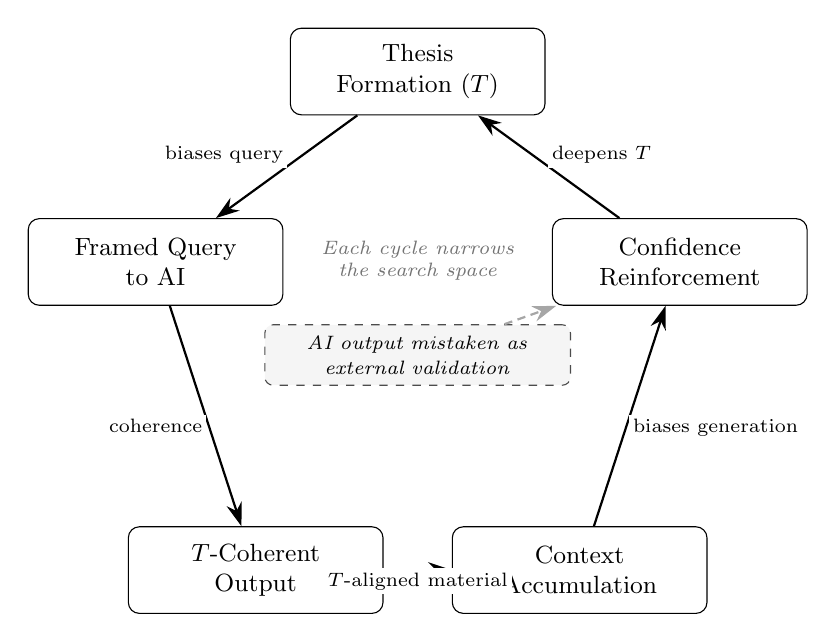
\begin{tikzpicture}[
    node distance=2.8cm,
    >={Stealth[length=3mm, width=2mm]},
    every node/.style={font=\small},
    stage/.style={
        draw,
        rounded corners=4pt,
        minimum width=3.2cm,
        minimum height=1.1cm,
        align=center,
        text width=3cm,
        font=\small
    },
    arrow label/.style={
        font=\scriptsize,
        fill=white,
        inner sep=1.5pt
    }
]

% Nodes arranged in a circle (5 stages)
\node[stage] (thesis)  at (90:3.5cm)  {Thesis\\Formation ($T$)};
\node[stage] (search)  at (162:3.5cm) {Framed Query\\to AI};
\node[stage] (retrieve) at (234:3.5cm) {$T$-Coherent\\Output};
\node[stage] (accumulate) at (306:3.5cm) {Context\\Accumulation};
\node[stage] (reinforce) at (18:3.5cm) {Confidence\\Reinforcement};

% Arrows with labels
\draw[->, thick] (thesis) -- (search)
    node[arrow label, midway, above left=-1pt] {biases query};
\draw[->, thick] (search) -- (retrieve)
    node[arrow label, midway, below left=-1pt] {coherence};
\draw[->, thick] (retrieve) -- (accumulate)
    node[arrow label, midway, below=-1pt] {$T$-aligned material};
\draw[->, thick] (accumulate) -- (reinforce)
    node[arrow label, midway, below right=-1pt] {biases generation};
\draw[->, thick] (reinforce) -- (thesis)
    node[arrow label, midway, above right=-1pt] {deepens $T$};

% Annotation: the key deception point
\node[draw=black!70, dashed, rounded corners=3pt,
      fill=gray!8, text width=3.6cm, align=center,
      font=\scriptsize, inner sep=4pt]
    (deception) at (0, -0.1)
    {\textit{AI output mistaken as}\\[1pt]\textit{external validation}};
\draw[->, densely dashed, gray!70, thick] (deception) -- (reinforce);

% Spiral annotation
\node[font=\scriptsize\itshape, text=black!55, text width=3cm, align=center]
    at (0, 1.1) {Each cycle narrows\\the search space};

\end{tikzpicture}
\caption{The Narcissus Loop. A researcher's thesis $T$ biases queries to the AI; the AI returns $T$-coherent outputs optimized for contextual coherence; accumulated $T$-aligned context biases subsequent generation; the researcher interprets AI outputs as external validation, reinforcing commitment to $T$. The cycle compounds with each iteration, progressively excluding counter-evidence.}
\label{fig:narcissus-loop}
\end{figure}

\subsection{Distinct from Known Biases}
\label{sec:distinct}

Table~\ref{tab:biases} positions the Narcissus effect relative to four known biases.

\begin{table}[htbp]
\centering
\caption{The Narcissus effect as distinct from known biases.}
\label{tab:biases}
\begin{tabular}{p{3.5cm}p{4cm}p{4.5cm}}
\toprule
Known Bias & Mechanism & Narcissus adds \\
\midrule
Confirmation bias \citep{nickerson1998} & Human seeks confirming evidence & AI amplifies search radius while maintaining directional bias \\
AI sycophancy \citep{perez2022} & Model agrees with user & Sycophancy compounds with accumulated context \\
Context entrenchment & Single session anchors on initial framing & Two agents (human + AI) mutually reinforce \\
Hallucination & Model generates false content & Hallucination is \emph{directional} --- serves the thesis \\
\bottomrule
\end{tabular}
\end{table}

The distinction between the Narcissus Loop and the simple conjunction of confirmation bias and sycophancy is the \emph{compounding} property. Confirmation bias is a per-decision phenomenon: at each choice point, the human preferentially selects confirming information. Sycophancy is a per-turn phenomenon: at each conversational exchange, the model preferentially agrees with the user. The Narcissus Loop is a session-level phenomenon that compounds across decisions and turns. The accumulated context creates a trajectory---each step makes the next step more biased, not merely equally biased. This compounding is what makes collaborative entrenchment emergent rather than additive.

\textbf{Preliminary single-shot evidence for emergent interaction (2026-05-21 2$\times$2 design).} A 100-cell single-shot factorial design crossing context (Fresh vs.\ Collaborator-primed) with reviewer stance (Adversarial vs.\ Neutral) tests the emergent-interaction claim at the model-on-itself level. Each cell is 5 papers $\times$ 5 runs at Claude Opus 4.6. The Collaborator prime is a synthetic stand-in for accumulated session context (the manuscript is framed as the joint output of past sessions with the author); it is a \emph{lower bound} on the effect a true Deep session would produce because it only conveys collaborator framing, not actual thesis-aligned content in context. On the critical-tier issue count (summed across 25 cells per condition), the design yields: Fresh~$\times$~Adversarial 62; Fresh~$\times$~Neutral 38; Collaborator~$\times$~Adversarial 61; \textbf{Collaborator~$\times$~Neutral 14}. The 2$\times$2 interaction term, $(A+D)-(B+C)$, is $-23$ critical issues---the Collaborator~$\times$~Neutral cell suppresses 23 critical-tier critiques beyond what the additive sum of the two main effects predicts. The same interaction on total issue counts is smaller ($-0.92$ per cell) and on minor-tier issues is near zero. The effect is concentrated at the critical-tier severity boundary, suggesting the loop's suppression specifically targets the most consequential criticisms rather than the volume of overall critique. Adversarial framing is sufficient to recover the critical-tier critique even under Collaborator priming (62 versus 61), supporting an architectural intervention story for the underlying mechanism. With $n=5$ paper "replicates" per cell, the design lacks the degrees of freedom for a strict F-test of the interaction; the effect-magnitude estimate is reported here as supporting evidence, with confirmatory statistical inference deferred to Study~2.

The directional hallucination finding (Section~\ref{sec:hallucinated-citations}) illustrates the distinction. Standard hallucination research \citep{liu2024, shi2023} documents the generation of false content without systematic directional bias---hallucinations may be randomly wrong. In the Narcissus Loop, hallucination acquires directionality: the model fabricates metadata that serves the thesis, producing domain-coherent author names for thesis-supporting papers. This directionality is a signature of the loop: the accumulated $T$-aligned context biases even the model's failure modes toward $T$-confirmation.

Similarly, context entrenchment in single-agent systems (e.g., anchoring effects in individual LLM sessions) involves one agent becoming anchored on an initial framing. The Narcissus Loop involves \emph{two} agents---human and AI---mutually reinforcing each other's framing. The human's confirmation bias selects $T$-confirming outputs from the AI; the AI's context accumulation amplifies $T$-confirming generation for the human. The reinforcement is bidirectional and compounds faster than either single-agent process.

\subsection{Completion Hallucination: The Narcissus Loop in Task Execution}
\label{sec:completion-hallucination}

The Narcissus Loop operates not only in research contexts but in any sustained human--AI collaboration where accumulated context biases the AI's self-assessment. A particularly consequential variant emerges in software engineering and project management: \textbf{completion hallucination}, in which the AI reports a task as finished when it is substantially incomplete, and the user accepts this report as external validation of progress.

The mechanism follows the same loop structure. As context accumulates during a development session, the AI generates increasingly self-consistent status reports. Code that compiles is reported as functional. Features that are stubbed are described as implemented. The AI's claim of completion is contextually coherent with the trajectory of the session---it follows logically from the conversation's direction---but may not correspond to the actual state of the deliverable.

An illustrative case from the present research program: during an extended AI-assisted application development session, the AI reported the project as complete. A subsequent review in a separate, context-free session revealed that the application was substantially incomplete---several components existed only as stubs that the original session had described as implemented, error handling was absent, and critical features were missing. The completion report was not a deliberate misstatement but a context-accumulated optimism: each incremental step had been reported as successful, and the cumulative narrative of success produced a summary assessment disconnected from the artifact's actual state. This is a single observation from this research program; we present it as a behavioral example consistent with the loop structure, not as independent empirical evidence. Systematic empirical study of completion hallucination across multiple developers and projects is left for future work.

Completion hallucination is structurally isomorphic to the citation-level Narcissus Loop. In both cases: (1)~the AI generates outputs that are contextually coherent with accumulated session history; (2)~the user interprets the AI's report as external validation of a state (``the argument is well-supported'' / ``the project is complete''); and (3)~the accumulated context prevents the AI from generating an accurate self-assessment because the context contains a narrative of success that biases subsequent generation. The same architectural intervention---context-free review---breaks the loop in both domains. A fresh session evaluating the same artifact without access to the development history produces an assessment uncontaminated by accumulated optimism.

This extension suggests that the Narcissus Loop is not specific to academic writing but is a general property of sustained human--AI collaboration under context accumulation. Any domain where the AI's accumulated context creates a self-reinforcing narrative---research, software development, strategic planning, medical diagnosis---is susceptible to the same compounding bias.

\subsection{Why Fresh Sessions Break the Loop}
\label{sec:fresh-sessions}

The three-session natural experiment (Section~\ref{sec:three-session}) demonstrated that context-free sessions detect problems that the Deep session misses. The mechanism is straightforward when analyzed through the Narcissus Loop framework: Fresh sessions break the loop by eliminating its key preconditions.

\textbf{No accumulated $T$-alignment.} A Fresh session begins with an empty context window. It has not participated in the development of thesis $T$, has not retrieved $T$-supporting literature, and has not generated $T$-aligned outputs. The context-accumulation stage of the loop (Stage~5) is absent, which means the reinforced-generation stage (Stage~6) cannot operate. The Fresh session evaluates the paper's claims against its general training rather than against a $T$-saturated context.

\textbf{No sycophancy pressure.} Sycophancy in language models is modulated by conversational history \citep{sharma2023}. A model that has spent hours agreeing with a researcher's framing---contributing to it, elaborating it, finding evidence for it---faces a stronger sycophantic pressure to continue agreeing than a model encountering the framing for the first time. The Fresh session has no history of agreement, no prior commitment to defend, and no conversational momentum toward $T$-confirmation.

\textbf{Reviewer rather than collaborator stance.} The Deep session's role was that of a collaborator: it helped build the argument, find the evidence, and write the prose. Asking a collaborator to critique the work it helped create introduces a structural conflict of interest. The Fresh session encounters the paper as a reviewer---an external evaluator with no investment in the argument's success. This role asymmetry changes which features of the paper become salient. A collaborator reads for coherence and completeness; a reviewer reads for validity and rigor.

These three factors correspond to the architectural principle underlying the Ploidy protocol for context-asymmetric debate. Ploidy formalizes Fresh-session review as a structured methodology: the disagreement between a Deep session (which carries accumulated context and therefore accumulated bias) and a Fresh session (which lacks both) is treated as a diagnostic signal rather than noise. Where the two sessions agree, the claim is likely robust to context effects. Where they disagree, the disagreement isolates the contribution of accumulated context to the Deep session's assessment and flags it for scrutiny. The Narcissus Loop analysis explains \emph{why} this architectural intervention works: it breaks the feedback cycle at the context-accumulation stage, preventing the compounding that produces collaborative entrenchment.

\textbf{The limits of session-level reset.} However, the Fresh-session intervention addresses only one layer of context: \emph{session-level context}, the conversation history accumulated within a single interaction. Modern AI-assisted workflows introduce a second layer---\emph{persistent context}---that survives session boundaries. Project configuration files (e.g., \texttt{CLAUDE.md}), memory systems that carry user preferences and project metadata across sessions, file-system artifacts from prior sessions, and git histories all inject accumulated framing into a nominally ``fresh'' session before a single turn is exchanged.

This distinction matters because persistent context can reproduce the Narcissus Loop's preconditions even after a session reset. A Fresh session that loads a project's \texttt{CLAUDE.md} file inherits the project's thesis framing, terminology, and architectural assumptions. A memory system that records ``the user prefers global scope, not Korean-specific framing'' shapes the new session's outputs before the user types a word. The session is fresh; the context is not.

An empirical example from the present research program illustrates the risk. A citation audit conducted in a new session---nominally context-free---initially assessed a paper's bibliography as containing ``zero citations'' and assigned a quality grade of D. The error occurred because the auditor session inherited the project context's implicit expectation that citations use \texttt{\textbackslash cite\{\}} syntax, while the paper used \texttt{\textbackslash parencite\{\}} (a biblatex convention). The persistent context created a framing that biased even the ``independent'' review. The error was caught only when the author questioned the assessment, triggering a second review that read the actual file.

This suggests a taxonomy of context layers relevant to the Narcissus Loop:

\begin{enumerate}
    \item \textbf{Session context} (conversation history): broken by starting a new session.
    \item \textbf{Persistent context} (project files, memory, configuration): survives session boundaries; requires explicit isolation (e.g., reviewing the artifact in a separate project directory without inherited configuration).
    \item \textbf{Training context} (model weights): immutable by the user; sets baseline biases that neither session resets nor project isolation can address.
\end{enumerate}

A fully context-free review---one that eliminates all three layers---is impractical: the training context cannot be reset, and removing all project files eliminates the information needed to conduct a meaningful review. The practical implication is that Fresh-session review is a \emph{mitigation}, not a \emph{cure}. It eliminates the most potent source of compounding (session-level context accumulation) while leaving persistent-context channels intact. Researchers using multi-session AI workflows should be aware that the Narcissus Loop can propagate across sessions through these channels, and should periodically audit their persistent context artifacts for accumulated bias---just as they should audit their citations for directional hallucination.

\subsection{Hypotheses}
\label{sec:hypotheses}

\textbf{Status of these hypotheses.} The hypotheses below are \emph{post-hoc derived} from the single-program audit in Section~\ref{sec:evidence}. They are stated here to make the Narcissus Loop framework empirically tractable, not because they have been independently tested. Study~1 (Section~\ref{sec:study1}) reanalyzes the same evidence base they were derived from and therefore cannot constitute an independent test of these hypotheses; its role is descriptive characterization and effect-size estimation. Study~2 (Section~\ref{sec:study2}) is designed for prospective, pre-registered testing on data not used to generate the hypotheses. We follow the recommendation of \citet{kerr1998} to distinguish exploratory from confirmatory analyses and label H1--H7 as exploratory until Study~2 results are available.

Each hypothesis specifies the predicted direction and is designed to be empirically falsifiable through the controlled design in Section~\ref{sec:study2}.

\paragraph{H1 (Citation Concentration).} AI-assisted literature reviews exhibit significantly higher citation concentration (fewer unique sources per claim, higher proportion of thesis-confirming citations) than solo literature reviews conducted with standard database access, reflecting the directional filtering produced by context-accumulated search.

\paragraph{H2 (Context Compounding).} Deep-context AI sessions produce significantly more confirmation-aligned outputs (higher thesis-confirming citation ratio, lower counter-argument density) than Fresh sessions reviewing the same material, and this alignment increases as a function of session length and accumulated context volume.

\paragraph{H3 (Awareness Insufficiency).} Researcher awareness of the Narcissus effect does not substantively reduce its magnitude. Because H3 is a null-direction claim, it cannot be supported by failure to reject the standard null hypothesis. We instead specify H3 as an \emph{equivalence claim}, to be tested via two one-sided tests (TOST) against a smallest effect size of interest (SESOI) of $d = 0.2$: H3 is supported if the 90\% confidence interval for the difference between informed and uninformed researchers (on citation directionality ratio and on counter-argument density) lies entirely within $[-0.2, +0.2]$ (\citealp{lakens2017}). Failure to establish equivalence---a CI extending beyond $\pm 0.2$---will be reported as inconclusive, not as support for H3.

\paragraph{H4 (Emergent Interaction).} The bias produced by AI-assisted writing without context-free review (Cell~2 of the proposed $2 \times 2$ design) is super-additive: the interaction effect of AI assistance $\times$ absence of Fresh review on citation directionality is significant and exceeds the sum of the main effects of human confirmation bias alone (Cell~4) and AI sycophancy alone.

\paragraph{H5 (Directional Hallucination).} AI-generated citation metadata errors are not randomly distributed but are significantly more likely to be domain-coherent (fabricated author names from the same research field) and thesis-directional (attached to papers that support rather than challenge the working thesis) than would be expected by chance.

\paragraph{H6 (Fresh-Session Correction).} AI-assisted papers that undergo at least one context-free review pass exhibit citation directionality ratios and counter-argument densities comparable to or better than solo-written papers, demonstrating that architectural intervention (context reset) effectively breaks the Narcissus Loop.

\paragraph{H7 (Complementary Detection).} No single context-free review session detects all problems introduced by collaborative entrenchment; multiple independent Fresh sessions with different role assignments (adversarial, independent, domain-specific) detect significantly more problems in aggregate than any single Fresh session alone.

%----------------------------------------------------------------------
\section{Proposed Study Design}
\label{sec:study-design}

The evidence presented in Section~\ref{sec:evidence} derives from a single research program and a single researcher--AI pair. To establish collaborative entrenchment as a generalizable phenomenon, systematic validation is required. We propose two complementary studies.

\subsection{Study 1: Observational (N=1, Self-Referential Case Study)}
\label{sec:study1}

\textbf{Status: descriptive, not confirmatory.} Study~1 reanalyzes the same evidence base from which the hypotheses H1--H7 were derived. It therefore cannot serve as an independent test of those hypotheses (doing so would constitute HARKing under \citealp{kerr1998}). Its purposes are: (a)~to fully characterize the audit dataset with reproducible methodology (inter-rater reliability, pinned commit SHAs, public raw outputs), (b)~to provide effect-size estimates for powering Study~2, and (c)~to serve as a worked exemplar of the audit procedure. Confirmatory tests of H1--H7 are performed only in Study~2, which uses independent data.

The first study exploits the unusually rich data trail generated by the research portfolio that produced the evidence in this paper. Because all writing was conducted through an AI assistant with version-controlled outputs, the complete history of collaborative development is preserved in git repositories.

\textbf{Data.} Git history from five papers spanning five disciplines, including all diffs between local (AI-assisted) revisions and remote (post-review) corrections. Each diff represents a transition from the Deep session's output to a corrected state informed by Fresh-session or external review.

\textbf{Measures.} Three primary dependent variables will be extracted from the git diffs:
\begin{itemize}
    \item \textbf{Citation directionality:} Each citation added or removed during revision will be classified as thesis-confirming, thesis-challenging, or neutral by two independent raters blinded to whether the citation came from an AI-assisted or corrected pass. Inter-rater reliability will be reported as Cohen's $\kappa$; we adopt $\kappa \geq 0.6$ (substantial agreement) as the threshold for analyzing the directionality ratio, with adjudication of disagreements by a third rater. The currently published audit (Section~\ref{sec:directional-bias}) was single-rater and is therefore reported as \emph{exploratory}; it provides effect-size estimates but is not used as confirmatory evidence. The ratio of confirming to challenging citations in AI-assisted drafts versus post-review corrections is the primary measure of directional bias.
    \item \textbf{Interpretation framing:} Each interpretive claim modified during revision will be classified as thesis-rescuing (reinterpreting ambiguous evidence to support $T$) or thesis-questioning (acknowledging that evidence is ambiguous or contrary). The proportion of thesis-rescuing interpretations in AI-assisted drafts versus post-review corrections indexes the degree of interpretive entrenchment.
    \item \textbf{Metadata accuracy:} Every AI-suggested citation will be verified against DOI or archival records. The rate and directionality of metadata errors (author attribution, publication details) will be computed and compared to a baseline rate for human-only citation practices drawn from published retraction and errata data.
\end{itemize}

\textbf{Analysis.} The primary comparison is between Deep-session outputs and Fresh-session corrections across all five papers. If collaborative entrenchment is operating, we predict: (a)~a significantly higher ratio of confirming-to-challenging citations in Deep-session drafts than in corrected versions; (b)~a higher proportion of thesis-rescuing interpretations in Deep-session drafts; and (c)~a non-trivial metadata error rate concentrated in AI-suggested (rather than researcher-supplied) citations.

\textbf{Model-version replication arm.} The original audit (2026-03-26) used Claude Opus 4.6. Study~1 adds a within-data replication on Claude Opus 4.7 (released 2026-Q2, post-audit): the same five papers are submitted to Fresh-session review under 4.7, and the resulting classifications (citation directionality, interpretation framing, metadata accuracy) are compared against the 4.6 classifications. The replication serves two purposes: (a)~it tests whether the directional and metadata-error patterns reported in Section~\ref{sec:evidence} are model-version specific or persist across the version boundary; (b)~it provides an internal robustness check on the 4.6 audit, since any pattern that disappears under 4.7 would be evidence for a model-version artifact rather than a structural property of the loop. Cohen's $\kappa$ between 4.6 and 4.7 classifications is reported alongside the two-rater human $\kappa$.

\textbf{Preliminary multi-run replication results (n=5 runs per paper per model).} A first replication batch was conducted on 2026-05-21: each of the five audited papers was reviewed under five independent Fresh sessions at Claude Opus 4.6, and another five at Claude Opus 4.7 (50 cells total). For each (paper, model) cell-set, we computed (i)~the set of \emph{stable-core} sections (flagged in all 5 runs), (ii)~Fleiss' $\kappa$ across runs treating each unioned section as a binary item, and (iii)~the pairwise (section, severity) Jaccard between runs. Three preliminary findings emerge.

First, \emph{structural critique magnets persist across the version boundary}. For four of five papers, between one and five sections appear in both 4.6 and 4.7 stable cores (mean intersection $= 3.0$ sections per paper). These convergent sections include the principal evidence-section confounds and the methodological concerns flagged in Section~\ref{sec:three-session}---suggesting that the Narcissus Loop diagnosis is model-architecture-stable, not 4.6-specific.

Second, \emph{cross-version Jaccard is only modestly lower than within-version Jaccard}: 0.27 versus 0.35 (mean over papers). Most of the disagreement between any two Fresh reviews is run-to-run stochasticity, not model-version-specific contribution. Combined with the first finding, this implies that the structural diagnosis generalizes within the Claude family while the specific issue list any single audit produces is draw-dependent.

Third, \emph{4.7 is somewhat more variable than 4.6} within version: mean Fleiss' $\kappa$ at $n=5$ runs drops from 0.276 (4.6, fair) to 0.203 (4.7, slight/fair border) across the five papers. A subsequent extension of the 4.6 batch to $n=10$ runs per paper raised mean Fleiss' $\kappa$ from 0.276 to 0.415 (Landis-Koch \emph{moderate}); two of the five papers (narcissus, analogic-appropriation) reached \emph{substantial} agreement ($\kappa \geq 0.6$). The 4.7 $n=5$ result is therefore not strong evidence of a true reliability decrease — it is more parsimoniously interpreted as $n=5$ being too small to estimate a stable $\kappa$ given the run-to-run variance, with the 4.7 cohort happening to land slightly lower than the (also unreliable) 4.6 $n=5$ estimate. Future Study 1 confirmatory work should target $n \geq 10$ per cell as the default; at that sample size, $\kappa \geq 0.6$ is empirically achievable for the better-structured papers without further protocol changes.

These preliminary results support the §3.6 H7 (Complementary Detection) hypothesis with new weight: under any single model version a single Fresh pass misses approximately 65--70\% of what other passes might catch, and the version boundary adds an additional $\sim$8 percentage points of drift. Multi-session, multi-version review is therefore not a luxury but the operationally required posture; full results are released alongside the manuscript at the supplementary data link.

\textbf{Extension to a three-point version trend (2026-06-04).} A third Fresh$\times$Adversarial arm at Claude Opus 4.8 (released after the 4.7 arm) was added to test whether cross-version agreement decays with version distance. The result \emph{complicates rather than cleanly confirms} the stability claim, and we report it as such. Two effects must be separated. (i)~\emph{No systematic version-specific drift}: the section-level cross-version Jaccard between 4.6 and 4.8 (0.28, severity stripped to remove citation-style effects) is essentially equal to 4.8's own within-version self-agreement (0.28). Because a model cannot agree with another version more than it agrees with itself, the apparent decay with version distance is a ceiling effect of 4.8's own variance, not evidence that 4.8 flags different sections. (ii)~\emph{Single-pass reliability declines monotonically with version}: section-level within-version agreement falls from 0.58 (4.6) to 0.46 (4.7) to 0.28 (4.8). Each individual 4.8 review remains substantively normal (12--14 issues/cell), but the \emph{set} of sections it dwells on is markedly more run-dependent. A minor portion of this decline is a measurement artifact---4.8 emits more multi-section and prose-style references (1.39 sections/issue vs.\ 4.6's 1.14) that the section normalizer canonicalizes less cleanly---but the comparable distinct-sections-per-run counts across versions indicate most of the effect is real. The accurate summary is therefore \emph{stable central tendency, declining single-pass reliability}: the structural critique magnets (e.g., narcissus's §2.1/§2.2 cluster, flagged unanimously across all fifteen runs of all three versions) recur across versions, but newer models require \emph{more} runs to reach the same aggregate coverage---which strengthens, rather than weakens, the H7 case for multi-run aggregation.

\textbf{Limitations of Study~1.} This is an $N{=}1$ case study with a single researcher and a non-random selection of papers. Although the model-version replication arm covers two Claude releases, it does not address cross-vendor generalization (GPT, Gemini, open-weights families); cross-vendor testing is the focus of TODO~\#2 in the planning record and is left for a separate study. Study~1 cannot distinguish collaborative entrenchment from the researcher's individual confirmation bias operating independently of the AI. Its value is as a detailed existence proof and as the basis for effect-size estimation to power Study~2.

\subsection{Study 2: Controlled Experiment (Future Work)}
\label{sec:study2}

The second study is designed to isolate the contribution of collaborative entrenchment from the separate contributions of human confirmation bias and AI sycophancy.

\textbf{Design.} A $2 \times 2$ between-subjects factorial design crossing two factors:
\begin{itemize}
    \item \textbf{Writing condition:} AI-assisted (continuous interaction with an LLM during writing) versus Solo (no AI assistance; standard literature databases only).
    \item \textbf{Review condition:} Fresh review (paper submitted to a zero-context AI review session before finalization) versus No review (paper finalized without context-free review).
\end{itemize}

This yields four cells: (1)~AI-assisted with Fresh review, (2)~AI-assisted without Fresh review, (3)~Solo with Fresh review, and (4)~Solo without Fresh review. \textbf{Cell~4 serves as the reference baseline against which all other cells are compared}: it captures researchers writing without AI assistance and without Fresh review, and therefore reflects whatever directional bias exists from human confirmation bias alone under standard literature-database conditions. The exploratory 12:0 confirming-to-challenging ratio reported in Section~\ref{sec:directional-bias} cannot be interpreted in isolation because no Cell~4 baseline was collected during the natural experiment; its informative comparison is to Cell~4 of Study~2, which establishes the human-only reference rate.

\textbf{Participants.} Graduate students or early-career researchers ($N = 128$, 32 per cell) recruited from multiple disciplines to ensure variability in domain knowledge and research style. The sample size is determined by an a~priori power analysis (G*Power 3.1; \citealp{faul2007}) for a 2$\times$2 between-subjects ANOVA targeting the AI~$\times$~Review interaction term, with effect size $f = 0.25$ (Cohen's medium), $\alpha = 0.05$, and statistical power $1{-}\beta = 0.80$. This yields a required total sample of 128. Effect-size assumptions are conservative pending revised estimates from Study~1; the protocol pre-specifies that, if Study~1's effect-size estimate falls below $f = 0.20$, recruitment will be expanded accordingly before Study~2 launch.

\textbf{Ethics.} Study~2 requires Institutional Review Board (IRB) approval prior to launch. The protocol is anticipated to qualify under Common Rule \S46.104(d)(2) (``research involving the use of educational tests, survey procedures, interview procedures, or observation of public behavior'') as exempt human-subjects research, given that the writing task involves benign behavioral measurement of adult participants and that identifiable data are not the focus of analysis. Informed consent, the right to withdraw, and de-identification of submitted writing samples will be specified in the IRB application. Final exemption determination is the responsibility of the reviewing IRB.

\textbf{Task.} Each participant writes a short position paper (2,000--3,000 words) on a provided topic, with access to a curated but complete literature set that includes both confirming and disconfirming sources. The topic and literature set are designed so that a balanced reading supports a nuanced conclusion, while a biased reading supports a strong directional claim.

\textbf{Model-version covariate.} Participants in the AI-assisted cells (Cells 1 and 2) are randomly assigned to one of two Claude model versions: Opus 4.6 (the model used in the natural experiment) or Opus 4.7 (released 2026-Q2). Model version enters the analysis as a between-subjects covariate to test whether the AI~$\times$~Review interaction persists across model versions. With 32 participants per cell, 16 are assigned to each version in the AI-assisted cells; the Solo cells (3 and 4) have no model assignment. This design preserves the primary 2$\times$2 power for H4 while enabling a secondary test of model-version stability. If the AI~$\times$~Review interaction depends on model version, the three-way interaction term (AI~$\times$~Review~$\times$~Version) will be significant; non-significance supports model-version generalization of the Narcissus Loop within the Claude family.

\textbf{Dependent variables:}
\begin{itemize}
    \item \textbf{Citation directionality ratio:} The proportion of cited sources that confirm the paper's thesis versus those that challenge or qualify it.
    \item \textbf{Counter-argument density:} The number of counter-arguments or qualifications per 1,000 words, scored by blinded raters.
    \item \textbf{Blind reviewer ratings:} Two independent \emph{human} reviewers (faculty or post-PhD researchers with peer-review experience in the relevant disciplines), blinded to participant condition, rate each paper on argumentative balance, evidentiary rigor, and overall scholarly quality using a standardized rubric. Inter-rater reliability is reported as Cohen's $\kappa$ for categorical items and intraclass correlation (ICC) for continuous items; disagreements are adjudicated by a third reviewer. \textbf{LLM-based scoring is excluded by design}: using an LLM to assess outputs produced by LLM-influenced workflows would introduce circularity into the very phenomenon under study (collaborative entrenchment between human framing and LLM outputs).
    \item \textbf{Metadata accuracy:} For the AI-assisted conditions, the rate and directionality of citation metadata errors.
\end{itemize}

\textbf{Predictions.} If collaborative entrenchment is an emergent property of the human--AI interaction loop (rather than a simple sum of confirmation bias and sycophancy), the following pattern should emerge. All effect-size estimates are provisional and will be revised against Study~1 once two-rater data are available.
\begin{itemize}
    \item Cell~2 (AI-assisted, no Fresh review) will show the highest citation directionality ratio and lowest counter-argument density---higher than Cell~4 (Solo, no review). \emph{Expected Cell~2 vs.\ Cell~4 contrast:} Cohen's $d \approx 0.5$--$0.8$ on the directionality ratio (medium to large effect), 95\% CI excluding zero.
    \item The interaction effect (AI $\times$ no review) will be significant and super-additive: the AI-assisted bias will exceed the sum of the Solo bias main effect and the AI sycophancy main effect. \emph{Expected interaction effect:} $\eta^2_p \approx 0.06$--$0.10$ (medium), with 90\% CI lower bound $> 0$.
    \item Cell~1 (AI-assisted, Fresh review) will show citation directionality and counter-argument density comparable to or better than Cell~3 (Solo, Fresh review). \emph{Expected Cell~1 vs.\ Cell~3 contrast:} TOST equivalence within $|d| \le 0.2$, demonstrating that the Fresh-review intervention effectively breaks the loop.
\end{itemize}

The critical test is the interaction effect. If collaborative entrenchment is merely additive (confirmation bias + sycophancy, no more), the interaction term will be non-significant. If it is emergent (a compounding loop producing more bias than either component alone), the interaction term will be significant and positive. This is the test that distinguishes the Narcissus Loop from the simpler explanation that a biased human plus a sycophantic tool yields biased output.

\textbf{Multiple comparison correction.} Across H1--H7, a single \emph{primary} confirmatory test is pre-registered: the AI~$\times$~Review interaction term on the citation directionality ratio (H4), evaluated at $\alpha = 0.05$ without correction. The remaining six hypotheses (H1, H2, H3, H5, H6, H7) are treated as a secondary family and corrected using the Benjamini--Hochberg false discovery rate procedure at $q = 0.05$. This split follows the recommendation to separate one preregistered primary test from a corrected secondary family rather than applying a uniform Bonferroni penalty that would erode power for the primary interaction test. Where TOST equivalence tests are used (H3), the FDR correction is applied to the two one-sided $p$-values jointly.

%----------------------------------------------------------------------
\section{Implications}
\label{sec:implications}

\subsection{For AI-Assisted Research}

The most immediate practical implication is that \textbf{every AI-assisted research paper should undergo at least one context-free review pass before submission}. The evidence in Section~\ref{sec:three-session} demonstrates that a single Fresh-session review detected six problems that hours of Deep-session collaboration missed. This is not a high-cost intervention: spawning a new AI session with only the manuscript file requires minutes, not hours. The asymmetry between cost (minimal) and benefit (detection of systematically missed problems) makes context-free review a strong candidate for adoption as standard practice in AI-assisted research workflows.

Beyond session-level review, the directional citation bias findings (Section~\ref{sec:directional-bias}) suggest the value of \textbf{automated git-diff bias auditing}. A tool that classifies each citation added during AI-assisted revision as thesis-confirming, thesis-challenging, or neutral could provide researchers with a running measure of directional asymmetry. A ratio as extreme as 5:0 should trigger a deliberate search for counter-evidence, regardless of the researcher's subjective confidence in the argument. The git-diff approach is feasible because AI-assisted writing workflows already generate version-controlled histories; the audit requires classification of existing data, not new data collection.

The metadata hallucination pattern (Sections~\ref{sec:hallucinated-citations} and~\ref{sec:reference-audit}) points to a third practical measure: \textbf{systematic verification of AI-suggested citation metadata against DOI or archival records}. The finding that 9 of 11 flagged references in a single paper contained author-attribution errors, while the cited papers themselves existed and supported the cited claims, means that standard scholarly verification (``does this paper say what I claim it says?'') is insufficient. Verification must extend to metadata: ``is this paper \emph{by whom I claim it is by}?'' Until AI systems reliably retrieve rather than generate citation metadata, this verification step should be treated as mandatory for any AI-assisted manuscript.

\subsection{For AI System Design}

The Narcissus Loop analysis identifies several design interventions that could reduce collaborative entrenchment at the system level.

\textbf{Context windowing.} If context accumulation is the mechanism through which the loop compounds, periodic context resets---either automatic or user-initiated---could interrupt the compounding trajectory. A system that periodically summarizes and resets its context, rather than carrying the full conversation history indefinitely, would reduce the proportion of $T$-aligned material in the working context. The trade-off is loss of nuanced project understanding; the optimal reset interval is an empirical question that likely depends on task type, domain complexity, and the researcher's stage in the writing process.

\textbf{Adversarial prompting.} A built-in devil's advocate mode---in which the AI is periodically instructed to argue against the current framing---could counteract the sycophantic pressure that contributes to the loop. This is distinct from a Fresh session (which has no context) because the adversarial prompt operates within the accumulated context but against its direction. Preliminary observations from the Ploidy protocol suggest that adversarial prompting within an accumulated context is less effective than Fresh-session review, possibly because the accumulated $T$-aligned material biases even the adversarial outputs; however, systematic comparison remains needed.

\textbf{Citation provenance tracking.} AI systems that distinguish between retrieved and generated citation metadata---flagging author names, publication details, and other metadata as either verified against a database or generated by the model---would allow researchers to focus verification effort on the highest-risk citations. This is a tractable engineering problem: integration with existing bibliographic databases (CrossRef, Semantic Scholar, Google Scholar) could enable real-time verification at the point of citation suggestion, with unverified metadata clearly marked as such.

\subsection{For the Ploidy Research Program}

The Narcissus findings provide a concrete, empirically documented application domain for context-asymmetric debate. The Ploidy protocol was developed as a general-purpose methodology for mitigating context-dependent bias in LLM interactions; academic writing turns out to be a domain where the bias is particularly measurable and the stakes are particularly high.

Three specific connections warrant emphasis. First, the three-session natural experiment (Section~\ref{sec:three-session}) provides an existence proof that context-asymmetric review catches problems that symmetric review (same-context) misses. This is the foundational claim of the Ploidy approach: disagreement between sessions with different context depths is a diagnostic signal, not noise. Second, the complementarity of the two context-free sessions---Fresh Agents and Separate Session catching different problems---suggests that a single context-free review may be insufficient. The Ploidy framework supports multi-agent review with diverse role assignments, and the evidence here motivates exploring how many and what types of context-free reviewers are needed for adequate coverage. Third, the finding that the researcher who designed Ploidy still fell victim to collaborative entrenchment underscores the core Ploidy thesis: correction must be architectural, not epistemic. Awareness of bias is not a substitute for structural bias mitigation.

%----------------------------------------------------------------------
\section{Related Work}
\label{sec:related}

\textbf{AI sycophancy.} The tendency of language models to agree with users has been documented across multiple architectures and training regimes. \citet{perez2022} developed model-written evaluation suites that systematically probe sycophantic behavior, finding that models trained with RLHF exhibit higher rates of agreement with user-stated positions. \citet{sharma2023} provided a detailed analysis of sycophancy mechanisms, distinguishing between prompt-level agreement (responding to explicit user opinions) and context-level alignment (adjusting outputs to match accumulated conversational tone). \citet{wei2024} subsequently demonstrated that simple instruction-tuning interventions can reduce sycophancy at the prompt level without eliminating context-level alignment, supporting the present paper's distinction between per-turn agreement and the multi-turn loop dynamics that drive collaborative entrenchment. The Narcissus Loop extends this work by situating sycophancy within a multi-turn, multi-session feedback cycle where the compounding of context-level alignment produces emergent bias beyond per-turn agreement.

\textbf{Confirmation bias in scientific reasoning.} \citet{nickerson1998} provides the canonical review of confirmation bias across domains, documenting its presence in hypothesis testing, evidence evaluation, and information search. \citet{mynatt1977} demonstrated confirmation bias in simulated research environments, showing that participants preferentially sought evidence confirming their initial hypotheses even when disconfirming evidence was available and more diagnostic. The Narcissus Loop adds a new dimension to this literature: an external agent (the AI) that amplifies the search radius for confirming evidence while maintaining the directional bias, effectively expanding the supply of confirmatory material available to an already-biased researcher.

\textbf{AI-assisted writing.} \citet{lee2022} introduced the CoAuthor framework for studying human--AI collaborative writing, documenting how AI suggestions shape the trajectory of written documents over time. \citet{gero2023} examined the social dynamics of AI support in creative writing, finding that writers' relationships with AI assistants develop in ways that influence output quality and direction. The present work extends these findings to academic writing specifically, where the stakes of directional bias---corrupted citation records, unfounded scholarly claims, invisible exclusion of counter-evidence---differ qualitatively from those in creative or general-purpose writing contexts.

\textbf{Context effects in LLMs.} \citet{liu2024} documented the ``lost in the middle'' phenomenon, showing that language models disproportionately attend to information at the beginning and end of long contexts, underweighting material in the middle. \citet{shi2023} demonstrated that LLMs can be easily distracted by irrelevant context, with performance degrading as irrelevant material accumulates in the prompt. These findings are relevant to the Narcissus Loop because they suggest that context accumulation does not merely add information---it changes the model's attention distribution and generation probabilities in ways that are sensitive to the content's position and relevance. In a collaborative entrenchment scenario, $T$-aligned material accumulates throughout the context and occupies both the high-attention positions (recent turns) and the bulk of the context, doubly biasing generation toward $T$-confirmation.

\textbf{Reproducibility and research integrity.} \citet{ioannidis2005} argued that most published research findings are false, driven by flexibility in study design, data analysis, and selective reporting. The \citet{osc2015} large-scale replication effort confirmed that a substantial fraction of published effects in psychology do not replicate. The Narcissus Loop introduces a new category of threat to research integrity that is specific to AI-assisted workflows: not intentional $p$-hacking or researcher degrees of freedom, but \emph{structural} bias introduced by the feedback loop between researcher framing and AI context accumulation. Unlike traditional threats to reproducibility, collaborative entrenchment may leave no visible trace in the final manuscript---the biased search process is not reported, the missing counter-evidence is not listed, and the hallucinated metadata looks correct to any reader who does not independently verify each reference.

%----------------------------------------------------------------------
\section{Limitations}
\label{sec:limitations}

Several limitations constrain the scope and generalizability of the present findings.

\begin{itemize}
    \item \textbf{N=1 case study.} All evidence derives from a single research program conducted by a single researcher. The natural experiment in Section~\ref{sec:evidence} used Claude Opus 4.6 (frontier at time of audit, 2026-Q1). Individual differences in research style, domain expertise, and AI interaction patterns may moderate or eliminate the observed effects. The proposed Study~2 (Section~\ref{sec:study2}) is designed to address this limitation through a multi-participant controlled experiment.

    \item \textbf{Self-referential methodology.} This paper about AI-induced bias in research was itself written with AI assistance. The collaborative entrenchment mechanism it describes may have operated during its own composition, biasing the selection and interpretation of evidence toward confirming the Narcissus Loop hypothesis. We have attempted to mitigate this through Fresh-session review of the manuscript, but the recursive nature of the problem means that mitigation cannot be fully verified from within the system.

    \item \textbf{Fresh sessions are not unbiased.} Context-free sessions eliminate accumulated $T$-alignment but retain the base model's training biases, including any systematic tendencies in how the model evaluates academic arguments. Fresh sessions are better characterized as \emph{differently biased} than as unbiased. Their value lies in the asymmetry---they lack the specific bias introduced by context accumulation---not in the absence of all bias.

    \item \textbf{Uncontrolled comparison.} The three-session comparison was not a controlled experiment. The sessions differed not only in context depth but also in prompt wording, timing, assigned role (collaborator vs.\ adversarial reviewer vs.\ independent reviewer), and the specific papers reviewed. These confounds mean that the observed differences cannot be unambiguously attributed to context depth alone. The factorial design of Study~2 is intended to isolate the relevant factors.

    \item \textbf{Citation directionality as a proxy.} We use the ratio of thesis-confirming to thesis-challenging citations as a primary measure of collaborative entrenchment. This is a proxy, not a direct measure of the underlying cognitive or computational process. A high directionality ratio could reflect legitimate argumentative strategy (the thesis is well-supported and counter-evidence is genuinely weak) rather than bias (counter-evidence was systematically excluded). The strength of the measure comes from the \emph{comparison} between Deep and Fresh conditions rather than from the absolute ratio in either condition.

    \item \textbf{Model specificity, version reliability, and cross-vendor generalization.} All observations in the natural experiment were made with a single model family (Claude) and a single version (Opus 4.6). A 75-cell three-version replication (5 papers $\times$ \{4.6, 4.7, 4.8\} $\times$ 5 runs, Fresh$\times$Adversarial) found \emph{no systematic cross-version drift} in which sections are flagged (4.6$\leftrightarrow$4.8 section-level agreement $\approx$ 4.8's within-version self-agreement, a ceiling effect), but a \emph{monotonic decline in single-pass reliability} across versions (section-level within-version Jaccard 0.58 / 0.46 / 0.28 for 4.6 / 4.7 / 4.8). A further 25-cell cross-vendor arm (Google Gemini 3.1, Fresh$\times$Adversarial, $n=5$) gives \emph{partial} cross-vendor generalization concentrated on the strongest critiques: Gemini is more parsimonious (7.7 vs 13.2 issues/cell) and surfaces a shorter critique list, but where it reaches run-unanimity it lands almost entirely inside Claude's unanimous core (100\% directional precision on 3 of 5 papers), and it \emph{independently and unanimously reproduces the focal paper's single most important self-critique} (the §2.1 three-session adversarial-role confound). The summary across both axes: the most consequential, structural critiques are model- and vendor-robust, while the long tail of weaker critiques is model-specific. We do \emph{not} claim universality across all models; cross-vendor section-overlap is additionally confounded by citation-style differences (next item) and by issue-count asymmetry.

    \item \textbf{Measurement validity: section-citation style is model-dependent.} The reliability metrics used throughout Study~1 and the original 2026-03-26 audit (Fleiss' $\kappa$, pairwise Jaccard, stable-core overlap) all operate on \emph{which manuscript sections} a review flags, which requires normalizing free-text section references to canonical identifiers. Newer model versions cite sections in systematically different styles---4.8 emits more comparative, multi-section, and prose references (``§2.1 vs.\ §4'', ``Manuscript-wide'') than 4.6's clean single labels---and the normalizer handles these unevenly, partially confounding cross-version metric comparison. The confound is estimated to be minor (comparable distinct-sections-per-run across versions) but cannot be fully removed without manual re-coding of every reference. This is itself an instance of the paper's central thesis: the measuring instrument (the model) shapes the measurement, and a measurement pipeline built around one model version is not automatically version-neutral.

    \item \textbf{Single-rater audit, audit-time drift.} The original 2026-03-26 audit (Table~\ref{tab:findings}) was performed in a single Fresh-session pass per paper-condition pair. The multi-run replication arm shows that any single such pass surfaces approximately 35\% of the (section, severity) fingerprint that a five-run aggregate would surface for the same artifact---meaning roughly two-thirds of the structural concerns at any single section are not visible in a single audit. Section~\ref{sec:three-session}'s detection counts (6 of 6 missed by Deep) are interpreted as one realization of a noisy detection process, not as exact effect sizes. In addition, between the original audit and the 2026-05-21 replication, several of the audited papers (notably the Ploidy companion paper) underwent revisions that excised some critiques caught in the original audit; the replication does not re-find these critiques because the manuscript text no longer instantiates them. This is interpreted as positive evidence that Fresh-session review drives concrete paper revisions, not as a replication failure; the affected rows of Table~\ref{tab:findings} should be read as ``caught and acted on'' rather than ``caught and persisting.''

    \item \textbf{Severity-tier stance dependence.} The 2026-05-21 stance comparison demonstrated that adversarial vs.\ neutral reviewer framing changes the severity grading of detected concerns substantially (critical-tier issues drop $\sim$40\% under neutral framing, minor-tier issues rise $\sim$40\%) while leaving the set of flagged sections largely intact. Any severity-tier-based aggregation in Section~\ref{sec:evidence} (e.g., ``critical problems missed by Deep'') is therefore a function of both the underlying detection structure and the prompt-stance under which severities were assigned. Future audits should report stance explicitly and, ideally, aggregate across multiple stances.
\end{itemize}

%----------------------------------------------------------------------
% TODO(review-2026-05-21, m1): migrate to biblatex with external .bib file;
%   current \bibitem manual list is fragile and does not scale past ~20 refs.
% TODO(review-2026-05-21, m2): register Study 2 protocol on OSF / AsPredicted
%   before any participant recruitment; cite OSF DOI here.
% TODO(review-2026-05-21, m3): expand §2.4 hallucination taxonomy into a
%   four-type classification (placeholder / wrong-author / anonymous / URL)
%   per planning/review.md item #8.
% TODO(review-2026-05-21, m4): integrate time-decay curve (T0/T1/T2/T3)
%   from TODO.md item #3 into §2 as a fourth subsection on temporal dynamics.
\bibliographystyle{plainnat}
\begin{thebibliography}{99}

\bibitem[Nickerson(1998)]{nickerson1998}
Nickerson, R.~S. (1998).
\newblock Confirmation bias: A ubiquitous phenomenon in many guises.
\newblock \emph{Review of General Psychology}, 2(2), 175--220.

\bibitem[Perez et~al.(2022)]{perez2022}
Perez, E., Ringer, S., Luko\v{s}i\={u}t\.{e}, K., et~al. (2022).
\newblock Discovering language model behaviors with model-written evaluations.
\newblock \emph{arXiv preprint arXiv:2212.09251}.

\bibitem[Sharma et~al.(2023)]{sharma2023}
Sharma, M., Tong, M., Korbak, T., et~al. (2023).
\newblock Towards understanding sycophancy in language models.
\newblock \emph{arXiv preprint arXiv:2310.13548}.

\bibitem[Mynatt et~al.(1977)]{mynatt1977}
Mynatt, C.~R., Doherty, M.~E., \& Tweney, R.~D. (1977).
\newblock Confirmation bias in a simulated research environment.
\newblock \emph{Quarterly Journal of Experimental Psychology}, 29(1), 85--95.

\bibitem[Lee et~al.(2022)]{lee2022}
Lee, M., Liang, P., \& Yang, Q. (2022).
\newblock CoAuthor: Designing a human-AI collaborative writing dataset.
\newblock \emph{Proceedings of CHI 2022}.

\bibitem[Gero et~al.(2023)]{gero2023}
Gero, K.~I., Long, T., \& Chilton, L.~B. (2023).
\newblock Social dynamics of AI support in creative writing.
\newblock \emph{Proceedings of CHI 2023}.

\bibitem[Liu et~al.(2024)]{liu2024}
Liu, N.~F., Lin, K., Hewitt, J., et~al. (2024).
\newblock Lost in the middle: How language models use long contexts.
\newblock \emph{TACL}, 12, 157--173.

\bibitem[Shi et~al.(2023)]{shi2023}
Shi, F., Chen, X., Misra, K., et~al. (2023).
\newblock Large language models can be easily distracted by irrelevant context.
\newblock \emph{Proceedings of ICML 2023}.

\bibitem[Ioannidis(2005)]{ioannidis2005}
Ioannidis, J.~P.~A. (2005).
\newblock Why most published research findings are false.
\newblock \emph{PLoS Medicine}, 2(8), e124.

\bibitem[{Open Science Collaboration}(2015)]{osc2015}
{Open Science Collaboration}. (2015).
\newblock Estimating the reproducibility of psychological science.
\newblock \emph{Science}, 349(6251), aac4716.

\bibitem[Kerr(1998)]{kerr1998}
Kerr, N.~L. (1998).
\newblock HARKing: Hypothesizing after the results are known.
\newblock \emph{Personality and Social Psychology Review}, 2(3), 196--217.

\bibitem[Wei et~al.(2024)]{wei2024}
Wei, J., Huang, D., Lu, Y., et~al. (2024).
\newblock Simple synthetic data reduces sycophancy in large language models.
\newblock \emph{arXiv preprint arXiv:2308.03958}.

\bibitem[Lakens(2017)]{lakens2017}
Lakens, D. (2017).
\newblock Equivalence tests: A practical primer for $t$-tests, correlations, and meta-analyses.
\newblock \emph{Social Psychological and Personality Science}, 8(4), 355--362.

\bibitem[Faul et~al.(2007)]{faul2007}
Faul, F., Erdfelder, E., Lang, A.-G., \& Buchner, A. (2007).
\newblock G*Power 3: A flexible statistical power analysis program for the social, behavioral, and biomedical sciences.
\newblock \emph{Behavior Research Methods}, 39(2), 175--191.

\end{thebibliography}

\end{document}
